\chapter{Literature Review}%
\label{chapter:literatureReview}

\begin{introduction}
The purpose of this chapter is to establish the theoretical and practical foundation for the development of the proposed solution. It begins by examining the vehicle maintenance process, highlighting its relevance to service quality and customer satisfaction. 

Then it incorporates real-world insights gathered from EMEL, the company responsible for operating Lisbon's Gira bike-sharing system. 

Next, it introduces the multiple concepts relevant to the thesis.

And finally, the chapter reviews existing software solutions in the market analyzing their strengths, limitations, and relevance to this dissertation.
\end{introduction} 

To gather relevant information for this topic, I conducted a literature search using the Scopus and Google Scholar platforms. In Scopus, I applied the query “\textit{Vehicle AND Maintenance AND Dealerships}”, which initially returned 49 papers. After a preliminary review of titles and abstracts, 24 were identified as potentially relevant. However, a closer analysis revealed that only three were directly applicable to this dissertation. Many of the discarded papers treated dealerships primarily as sales units of larger companies, which lies outside the scope of this work. Others focused on narrow applications of machine learning, such as predictive maintenance. While valuable in their own right, these approaches did not align with the dissertation's emphasis on web applications and maintenance process management.

A complementary search on Google Scholar yielded three additional studies related to the electric vehicle market in China. Although these works provided useful insights into international contexts, they were excluded as the focus of this dissertation is on maintenance operations rather than market-specific trends.

Ultimately, three papers were selected for detailed analysis. Two of them examined the vehicle maintenance process and highlighted the importance of service quality in ensuring customer satisfaction. The third presented a practical software solution with a use case comparable to the objectives of this dissertation. Together, these studies helped to define the research context and identify key problems and solutions to address during the development phase.

\section{Theoretical Concepts}

\subsection{Vehicle Maintenance}

Delivering vehicle maintenance services involves numerous activities, each crucial for maintaining service quality and ensuring customer satisfaction. 
Any deviation from these activities can negatively impact quality, leading to client dissatisfaction and loyalty loss. ~\cite{Setting_the_after_sale_process}
The loyalty of the client is the main source of income for the company, so it is important to maintain the quality of the service. ~\cite{Setting_the_after_sale_process}
To fulfill this requirement to the fullest, one must supervise every stage of the process. ~\cite{Setting_the_after_sale_process}


\begin{figure}[h]
  \caption{Macro-level Flow of a vehicle maintenance or repair service. This figure was inspired by figure 6: After Sales process from ~\citet{Setting_the_after_sale_process}.}
  \centering
  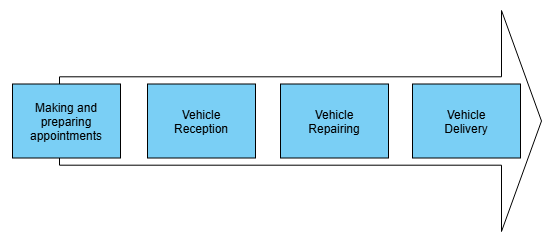
\includegraphics[width=0.50\textwidth]{figs/Vehicle_maintenace_macro}
  \label{fig:Vehicle_maintenace_macro}
\end{figure}

The general flow of vehicle maintenance is illustrated in the figure \ref{fig:Vehicle_maintenace_macro}. 
The first step of the process starts with a client interacting with the garage to schedule a vehicle maintenance or repair. 
After that, the client goes to the garage, where the receptionist receives the client and the vehicle.
Here, the mechanic will perform the maintenance of the vehicle and, when is done, the vehicle will be delivered to the client.

To ensure quality in the first step the receptionist must understand the fill capacity of the garage and the time to complete the job. 
With this information, the rececionist may accurately indicate the time to conclude the vehicle maintenance and get the client trust. ~\cite{Setting_the_after_sale_process}

In the second step, the receptionist and service advisor, when receiving the vehicle, must do a visual confirmation of the vehicle's condition. ~\cite{Setting_the_after_sale_process}
In this step, the receptionist explains to the client the services of the garage and they both agree with the services to be performed until a determined date. ~\cite{Setting_the_after_sale_process}

Following begins the third step and most important phase, the mechanic will perform the maintenance and repair of the vehicle. 
All of this process must be supervised by quality control to ensure that the job is done correctly. ~\cite{Setting_the_after_sale_process}
This includes the repair process, extra work, final tests, and service report. ~\cite{Setting_the_after_sale_process}
To accomplish that the use of a checklist is recommended to ensure precision and accuracy at each step. ~\cite{Setting_the_after_sale_process}

Finally, the last step is the delivery of the vehicle to the client. 
Here, the workshop manager must review the work done and the final price of the service to avoid extra payments from the client and incomplete payments to the workers. ~\cite{Setting_the_after_sale_process}

In this sense, the application of this dissertation will obey this flow.
For the receptionist and mechanic, the application will focus on reducing their mistake by giving accurate and illustrated information and making the work more effective.
And for the workshop manager to control the quality of the service with the assignment of tasks and authorization of purchases. 
Another user will be inserted into this flow, the warehouse operator, to manage the inventory of the dealership. 
The entire flow will be explained in Chapter III. 


\subsection{EMEL}


In June, I visited the company \ac{emel}, an entity responsible for operating and managing the public bike-sharing system Gira in Lisbon. This system comprises approximately 1,800 bicycles and 159 stations, supporting on average 7,405 trips per day, according to 2024 data ~\cite{Gira_Trips}. Each bicycle is scheduled for preventive maintenance either every 50 trips or every 14 days which results in an average of around 70 maintenance operations per day ~\cite{Gira_Maintenance}. This scale of demand requires a well-structured maintenance operation to ensure safety, reliability, and service availability.

To handle this demand, \ac{emel} follows a maintenance workflow that begins when a redistributor identifies a malfunction during routine operations and delivers the vehicle to the workshop. At this stage, the redistributor completes a paper form (Figures \ref{fig:emel_front} and \ref{fig:emel_back}), recording the detected faults and performing a simple diagnostic of electrical components such as the GPS unit and battery. If the vehicle fails these initial tests, it is set aside for a specialist to address before proceeding to standard maintenance. Otherwise, it enters a waiting list until a mechanic becomes available.

When a mechanic is free, the bicycle undergoes repair for both the reported issues and any additional problems detected during inspection. Upon completion, the mechanic records the parts used on the reverse side of the form. The bicycle is then forwarded to a quality control worker for validation. If defects are detected at this stage, the bicycle is returned to the same mechanic for correction before re-entering circulation. Although this process ensures that urgent faults are addressed, the high daily volume of bicycles forces \ac{emel} to prioritize speed over thoroughness, which can result in superficial inspections and undetected secondary issues.

These operational pressures also extend to inventory management. \ac{EMEL} collaborates with multiple suppliers under fixed contracts that specify delivery quantities and deadlines. This information is tracked manually through Excel spreadsheets, which are checked only at periodic intervals. This method provides limited insight into real-time consumption or future requirements. Without digital tools to integrate contract monitoring and inventory tracking, it becomes difficult to anticipate shortages or determine when new tenders should be initiated.

Introducing a digital system that integrates maintenance records with real-time inventory tracking would therefore enable \ac{emel} to optimize its resources, improve oversight, and maintain higher service quality despite the system's large operational scale.


\subsection{Computerized Maintenance Management System}

The software solution i will develop is a \ac{CMMS}.
A \ac{CMMS} is able to centralize and automate the management of maintenance operations, helping the dealership to manage the work tasks and the inventory, providing metrics to optimize the maintenance process.

It maintains a database with the information about the equipment, maintenance schedules, work orders, inventory, and personnel. 
It also document and reports all maintenance actions to facilitate the adherence to the regulatory standards ensuring the quality of the service. 
And analyzes the maintenance costs, downtime, efficiency, and other metrics to improve performence, optimization and reduce cost to the dealership.

The key benefits of the \ac{CMMS} are the improvement of the Preventive Maintenance, since it's easier to analyse the vehicle life and schedule a maintenance before the equipment failures occur; reduce costs, as the life of the vehicle is prolonged and the critical maintenace being avoided, this sofware provides a long-term cost saving; efficiency enhancement, by allowing the workers to focus on completing task instead of paperwork; and Regulatory Compliance, by keeping track and documenting the maintenance activities to comply by the organization standards. 

In conclusion, \ac{CMMS} provides a structured, data-driven approach to maintenance that enhances efficiency, reduces costs, ensures compliance, and ultimately supports the operational reliability of critical equipment and infrastructure.





\subsection{Service Quality}

Service quality is a critical factor in the success of vehicle maintenance services. One widely adopted framework for its evaluation is SERVQUAL, which provides a multidimensional approach for comparing consumers’ perceptions of service quality against their expectations. The model emphasizes five dimensions ~\cite{SERVQUAL_OLD}:


\begin{itemize}
   \item Tangibles – Physical facilities, equipment, and appearance of personnel.
   \item Reliability – Ability to consistently deliver services as promised.
   \item Responsiveness – Willingness to assist the customer and proactivity.
   \item Assurance – Demonstrate courtesy and knowledge and inspire trust and confidence.
   \item Empathy – Caring and treating customers as individuals.
  \end{itemize}

\begin{figure}[h]
  \caption{The 7-point Likert scale where the respondent may answer the question from strongly disagree to strongly agree. ~\cite{master_servqual_model}}
  \centering
  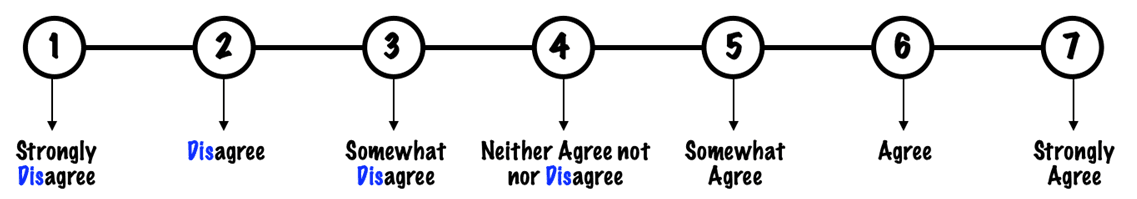
\includegraphics[width=\textwidth]{figs/likert_scale}
  \label{fig:likert_scale}
\end{figure}


To assess these dimensions, SERVQUAL relies on a questionnaire consisting of 22 items, divided across the five categories. Each item requires two ratings: one for the expectation of the service and another for the perception of the service received. The responses are given on a 7-point Likert scale, ranging from strongly disagree to strongly agree, as illustrated in Figure~\ref{fig:likert_scale} ~\cite{Measuring_After_sales_Service_Quality}. The quality gap is determined by the difference between the perception and expectation scores ~\cite{servqual_blog_da_qualidade} ~\cite{Measuring_After_sales_Service_Quality} ~\cite{SERVQUAL_OLD}.

An illustrative application of the SERVQUAL model can be found in the study by ~\citet{Measuring_After_sales_Service_Quality}, which assessed service quality at a CMV SA dealership in South Africa. The authors collected data through semi-structured questionnaires and interviews with customers, managers, and staff. The results, presented in Figure~\ref{fig:SERVQUAL_results}, revealed negative scores across all five dimensions, with an overall average gap of -0.10. These findings highlight that the services provided by the dealership consistently fell short of customer expectations. Among the main suggestions from customers were the expansion of workshops to reduce travel inconvenience and improving the availability of parts, which were often delayed due to international supply chains. The study underscores the importance of continuous service quality monitoring and recommends that dealerships regularly apply the SERVQUAL framework to identify and address performance gaps.

Building on this insight, this dissertation proposes the development of a client-facing application that enables users to evaluate the quality of service received, provide feedback, and make recommendations. This approach follows the SERVQUAL model and aims to strengthen customer trust and satisfaction.
\section{Existing solution}

\subsection{Fiix}
Fiix is a cloud-based \ac{CMMS} that allow organizations to manage their maintenance operations. 
It's main strengths lies on its advanced preventive maintenance scheduling, Comprehensive Work Order and Asset Management and AI-Powered Analytics and Reporting.

Despite the advantages of this software, Fiix has a high learning curve due to it's complexity and not intuitive old-fashion design interface. 
Also Fiix repordly lacks a built-in interal messaging system for crew communication. Most information sharing relies on notes and files attached to work orders, which may not be ideal for real-time collaboration.

With this effects in mind, i will aim in this software development to achieve a simple and user friendly solution where the users can intuitively interact with it by focusing on the key functional feature and easy navigation.

\subsection{Service Management for MAS Motors LLC}
MAS Motors LLC is a Toyota dealership in Libya that provides vehicle maintenance services. The company traditionally relied on manual processes, supported only by basic applications and paper-based documentation. While this approach was manageable at smaller scales, the expansion of the business exposed its inefficiencies and highlighted the need for a more modern solution ~\cite{MAS_MOTORS}. To address this challenge, ~\citet{MAS_MOTORS} developed a web application designed to streamline operations and enhance overall performance at the dealership.

The system was built to support multiple user groups—including service advisers, technicians, and customers—through a centralized platform that manages tasks such as job card handling, inventory updates, and customer service. The application was implemented using Laravel, a PHP web framework, together with MariaDB, an open-source relational database management system.

Evaluation results of the system were generally positive. A survey conducted with employees and customers assessed the solution using the \ac{FURPS} model, yielding scores of 4.27 for functionality, 4.30 for usability, 4.27 for reliability, 4.46 for performance, and 3.36 for supportability. While supportability received the lowest score—mainly due to limited configuration options ~\cite{MAS_MOTORS}—the system overall demonstrated clear improvements in service efficiency and customer satisfaction. Employees also provided valuable recommendations for future enhancements, including SMS-based service reminders, integration with social media platforms, and broader customer configuration options.

Building on these insights, my dissertation incorporates an email notification service, already used in the Lightmobie bike-sharing system, to handle alerts, user validation, and service-related notifications. This addition addresses part of the communication gap identified by MAS Motors employees while leveraging existing infrastructure within the Lightmobie ecosystem.

\subsection{Architecture Comparison}

The application will be developed using the ASP.NET Core MVC framework. This choice is motivated by several advantages over Laravel, the framework adopted in the solution proposed by ~\citet{MAS_MOTORS}. A detailed comparison between the two frameworks is presented in Table \ref{table:architetcture_comparison}.

One of the key advantages of ASP.NET Core MVC is its seamless integration with Microsoft SQL databases through the Entity Framework package, which greatly simplifies database interactions. While Laravel also supports relational database integration, ASP.NET Core MVC is generally more suitable for Microsoft environments ~\cite{asp_net_vs_laravel}.

In terms of performance, ASP.NET Core benefits from being based on C\#, a compiled language, whereas Laravel is built on PHP, an interpreted language. This distinction gives ASP.NET Core a performance edge, especially in applications that require scalability and responsiveness.

Security is another critical factor. Although Laravel provides features such as hashing and secure input validation, it requires deeper PHP expertise and continuous monitoring for vulnerabilities. ASP.NET Core, on the other hand, integrates more advanced security mechanisms out of the box, including role-based authentication and login management through the Identity Framework. These abstractions reduce the burden on the developer, allowing greater focus on application functionality ~\cite{asp_net_vs_laravel}.

\begin{table}[]
\begin{tabular}{| m{5em} | m{15em} | m{15em} |}
\hline
Parameter & Laravel & ASP.NET Core MVC \\
\hline
Language & PHP & C\# \\
\hline
Performance & Lower performance due to being an interpreted language & Higher performance due to being a compiled language \\
\hline 
Security & Provides features such as hashing and input validation, but requires strong PHP knowledge and manual management & Offers advanced built-in security tools, including role-based authentication and Identity Framework support \\
\hline
Integration with SQL & Supports various relational databases & Recommended for Microsoft environments due to strong integration packages \\
\hline
\end{tabular}
\caption{Comparison between Laravel and ASP.NET Core MVC frameworks for integration into the Lightmobie platform.}
\label{table:architetcture_comparison}
\end{table}
 
Another strong motivation for adopting ASP.NET Core MVC is its compatibility with Lightmobie's Fleet Management System, which follows the same architectural approach. This ensures easier integration, particularly for functionalities such as authentication and role assignment, which are already implemented and can be reused. While this choice may introduce some additional complexity, my prior involvement in developing the Fleet Management System provides familiarity with its features, thereby reducing the learning curve and facilitating a smoother integration process.
  

\section{Conclusion}

In this chapter i explained the theoretical concepts of the vehicle maintenance process in the literature and in the real case example EMEL in lisbon, and The SERVQUAL method to evaluate the quality of the service of a organization.
I also describe the existing solutions in the market, namely Fiix, and the results of MAS Motors LLC's application.
This solutions lack a intuitive interface and a notification service, so in this dissertation i will focus on accomplish that.

